\documentclass{note}
\usepackage[cpp,table]{mypackage}
\usepackage{footnote}
\makesavenoteenv{tabular}

\renewcommand{\thefootnote}{\fnsymbol{footnote}}

\title{模式识别笔记}
\author{陈鸿峥}
\date{{\builddatemonth\today}\protect\footnote{\text{Build \builddate\today}}} % protect!

\begin{document}

\maketitle
\renewcommand{\thefootnote}{\arabic{footnote}}
\setcounter{footnote}{0}

\setcounter{tocdepth}{2}%设置深度
\tableofcontents

\bigskip\bigskip

% !TEX root = main.tex

\section{计算机系统概述}
\subsection{计算模型}
\begin{itemize}
	\item 图灵机(1936)
	\item 冯诺依曼体系结构(1945)\footnote{非冯诺依曼体系结构:并行计算、量子计算、生物计算} --- 存储程序原理(\textbf{运算器}为中心)\\
	计算机采用\textbf{二进制}表示机器指令和数据,按照程序指令\textbf{顺序}执行
\begin{center}
\begin{tikzcd}
& & \text{存储器}\arrow{d} & & \\
\quad\arrow{r} & \text{输入设备}\arrow{r} & \text{运算器}\arrow{r}\arrow{d}\arrow{u} & \text{输出设备}\arrow{r} & \quad\\
& & \text{控制器}\arrow{u}\arrow{lu}\arrow{ru}\arrow[bend left]{uu} & &
\end{tikzcd}
\end{center}
而现在由于计算不是瓶颈,存储访问成为了瓶颈,故现代微机以\textbf{存储器}为中心
\begin{center}
\begin{tikzcd}
& & \text{运算器}\arrow{d} & & \\
\quad\arrow{r} & \text{输入设备}\arrow{r} & \text{存储器}\arrow{r}\arrow{d}\arrow{u} & \text{输出设备}\arrow{r} & \quad\\
& & \text{控制器}\arrow{u}\arrow{lu}\arrow{ru}\arrow[bend left]{uu} & &
\end{tikzcd}
\end{center}
\end{itemize}
[运算器、控制器](CPU)、存储器为计算机的核心,合称主机;外围设备,简称外设,指除主机外的其他设备,包括IO设备、外存等

计算机中的信息仍用二进制表示的原因:由物理器件性能决定
\begin{itemize}
	\item 二进制只有两种状态,容易找到具有2个稳定状态并且状态转换容易控制的物理器件(数字电路)
	\item 二进制编码运算规则简单
	\item 二进制的0、1与二值逻辑一致,容易实现逻辑运算
\end{itemize}
% There are two reasons computers use the binary system:
% 1.Two clearly distinct states that provide a safety range for reliability.
% 2.Least amount of necessary circuitry, which results in the least amount of space, energy consumption, and cost.

\subsection{计算机的发展历程}
按发展历程可分为:电子管、晶体管、集成电路、(超)大规模集成电路四代计算机
\par重大历史事件如下
\begin{center}
\begin{tabular}{|c|c|c|c|}
\hline
% 年份 & 姓名 & 事件 & 备注 \\
1904 & 弗莱明(Fleming) & 二极管 & \\\hline
1907 & 德福雷斯特(De Forest) & 三极管 & \\\hline
1938 & 香农(Shannon) & 布尔代数与二值电子器件(继电器) & 奠定数字电路基石 \\\hline
1946 & & 第一台通用计算机ENIAC & 十进制 \\\hline
1947 & \begin{tabular}{c}布莱顿(Brattain)\\
巴丁(Bardeen)\end{tabular} & 点接触晶体管 & \\\hline
1949 & 肖克利(Shockley) & 结型晶体管(1949) & 1956诺贝尔奖\\\hline
1950 & & 二进制和存储程序EDVAC & 实现冯诺依曼设想(组合进步) \\\hline
1958 & Jack Kilby & 集成电路 & 2000诺贝尔奖 \\\hline
1965 & Moore & 摩尔定律 & \begin{tabular}{c}
在价格不变的情况下,每18个月芯片上\\
晶体管数目翻倍,性能也提升一倍
\end{tabular}\\\hline
1971 & Intel & 第一款微处理器4004 & 10$\mu$m\\\hline
\end{tabular}
\end{center}

\subsubsection{单处理器(1971-2002)}
性能提升主要手段
\begin{itemize}
	\item 提升工作主频:KHz增长至GHz(生产工艺进步,流水线级数增加)
	\item 指令级并行(ILP)
\end{itemize}
\begin{proposition}[安迪-比尔定律]
Andy gives, Bill takes away. 安迪是原Intel CEO,比尔是原微软CEO,硬件厂商靠软件开发商用光自己提供的硬件资源得以生存
\end{proposition}
但遇到频率墙和功耗墙
\[\text{功耗(power)}\propto 1/2\times\text{CMOS电容}\times\text{电压}^2\times\text{转换(01)频率}\]
\par
2004年,Intel放弃4GHz Pentium4芯片开发,因无法解决散热问题,通过加快主频提升处理器性能的路走到尽头

\subsubsection{多核处理器(2005-)}
采用多核处理器不过是将硬件的问题丢到软件\footnote{“向多核的转变并不是因为我们在软件或体系结构技术上取得了中大突破而带来的。相反,这种转变是当单处理器体系结构发展遇到了难以克服的巨大障碍时,我们被迫作出的一种选择。”---Kurt Keutzer (UCB), \emph{The Landscape of Parallel Computing Research: A View from Berkeley}}
\begin{theorem}[阿姆达尔(Amdahl)定律]
\label{thm:amdahl}
\[\text{改进后的执行时间}=\text{受改进影响部分的执行时间}/\text{改进提高的倍数}+\text{不受影响的执行时间}\]
\[S_A=\frac{1}{s+(1-s)/N},\]
\end{theorem}
对计算机系统的某个部分采用并行优化措施后所获得的计算机性能的提高是有上限的,上限由串行部分所占的比例决定
\begin{theorem}[古斯塔夫森(Gustafson)定律]
\[S_G=(s'+p'\times N)/(s'+p')=N+(1-N)\times s',\]
其中,$s'$和$p'$为程序串行部分与可并行化部分在并行系统上执行的时间占总时间的比例,$N$为处理器数量,简便起见设总时间$s'+p'=1$
\end{theorem}
打破Amdahl定律\textbf{问题规模不变}的假设,任何足够大的任务都可以被有效地并行化,只要问题规模可扩展,并行所带来的加速比就可以扩展


\subsection{计算机系统的层次结构}
\begin{center}
\begin{tikzcd}
\text{高级语言层}\arrow{d}{}\\
\text{汇编语言层}\arrow{d}{}\\
\text{操作系统层}\arrow{d}{}\\
\text{指令系统层}\arrow{d}{}\\
\text{微体系结构层}\arrow{d}{}\\
\text{数字逻辑层}
\end{tikzcd}
\end{center}
程序编译运行过程:
\begin{center}
\begin{tikzcd}
\text{高级语言}\quad\arrow{r}{\text{预编译、编译}} & \quad\text{汇编语言}\arrow{r}{\text{汇编}} & \text{目标文件(二进制)}\arrow{r}{\text{链接}} & \text{可执行文件(二进制)}\arrow{d}{\text{加载}}\\
& & \text{电路上的电信号}\quad & \quad\text{二进制机器指令流(硬盘$\to$存储器)}\arrow[swap]{l}{\text{CPU取指译码}}
\end{tikzcd}
\end{center}
计算机内部工作过程:逐条执行加载到内存中的二进制机器指令流的过程

指令执行分为两个阶段,周期性重复性进行:
\begin{itemize}
	\item 取指阶段:CPU从内存中读取指令,程序计数器(PC)保存要被要被取出的\textbf{下一条}指令的地址,除非遇跳转指令,否则都加一个增量\footnote{程序计数器(Program Counter)是一个实际存在的寄存器吗? - Belleve的回答 - 知乎 \url{https://www.zhihu.com/question/22609253/answer/21965180} PC每次增加\textbf{一条指令的长度/寻址粒度},在MIPS中一条指令长4字节,寻址粒度1字节,故每次PC加4;而x86体系指令长度不定,每次增加量会变化}
	\item 执行阶段:对取出的指令译码后执行
\end{itemize}
软件系统可分为系统软件和应用软件

\subsection{计算机结构的八个想法}
\begin{enumerate}
	\item 摩尔(Moore)定律:集成电路资源每$18-24$个月翻倍
	\item 抽象(abstraction):简化设计
	\item 加速常用操作(Make common case fast):见定理\ref{thm:amdahl}
	\item 并行(parallelism)
	\item 流水线(pipelining)
	\item 预测(prediction)
	\item 内存等级制(hierarchy)
	\item 冗余实现可靠性(redundancy):检测故障及解决
\end{enumerate}

\subsection{基本指标}
表示计算机通信带宽时
\begin{center}
\begin{tabular}{ccccccc}\hline
KB(yte) & MB & GB & TB & PB & EB & ZB\\\hline
$10^3$ & $10^6$ & $10^9$ & $10^{12}$ & $10^{15}$ & $10^{18}$ & $10^{21}$\\\hline
\end{tabular}
\end{center}
表示计算机存储二进制时
\begin{center}
\begin{tabular}{ccccccc}\hline
KiB(yte) & MiB & GiB & TiB\\\hline
$2^{10}$ & $2^{20}$ & $2^{30}$ & $2^{40}$\\\hline
\end{tabular}
\end{center}
\begin{itemize}
	\item 位(bit/b):计算机处理、存储、传输信息的最小单位
	\item 字节(Byte/B) $1\text{ Byte}=8\text{ bit}$:现代计算机主存按字节编制,字节是最小可寻址单位
	\item 字(Word):表示被处理信息的单位,用来度量数据类型的宽度\footnote{字长是指CPU中\textbf{数据通路的宽度},等于CPU内部总线的宽度或运算器的位数或通用寄存器的宽度;字和字长的宽度可以一样,也可以不同,通常是字节的整数倍}
\end{itemize}
\par 一台32位的电脑,一个字等于4个字节,字长为32位;若字长为16位,则一个字等于2字节.
\par 4字节相当于8位16进制编码

\subsection{性能评价}
\label{subsec:performance}
CPU主频:对同一型号计算机,主频越高,完成指令一个执行步骤时间越短
\[\text{计算机的性能(Performance)}=1/\text{执行时间(Execution time)}\]
按照单位(量纲)进行换算即可
\[\begin{aligned}
\text{CPU执行时间(s)}&=\text{执行程序所需CPU时钟周期(cyc)}\times\text{时钟周期s/cyc)}\\
&=\text{指令数目(ins)}\times\text{CPI(cyc/ins)}\times\text{时钟周期(s/cyc)}
\end{aligned}\]
程序性能对执行事件的影响:
\begin{center}
\begin{tabular}{|c|c|c|c|}\hline
 & 指令数 & CPI & 时钟周期\\\hline
算法、编程语言、编译器 & $\times$ & $\times$ & \\\hline
指令集 & $\times$ & $\times$ & $\times$ \\\hline
计算机组成 & & $\times$ & $\times$ \\\hline
实现技术 & & & $\times$\\\hline
\end{tabular}
\end{center}
体系结构=指令集体系结构(功能定义与设计)+计算机组成(考虑用什么材料)\\
举例来说:
\begin{itemize}
	\item 指令集(ISA)考虑:是否提供乘法指令
	\item 组成(Organization)考虑:如何实现乘法指令(专门乘法器还是加法器+移位器)
	\item 实现技术(Technology)考虑:如何布线、用什么材料和工艺
\end{itemize}

% 带有处理器的设备一般称为智能化设备
% 完整的计算机系统应包括配套的硬件设备和软件系统
% !TEX root = main.tex

\section{贝叶斯决策论}
\subsection{离散变量}
处于类别$\omega_i$并具有特征值$x$,有后验概率\footnote{通常用$p(\cdot)$代表概率密度函数(连续变量),用$\pr{\cdot}$代表概率质量函数(离散变量)}
\[\prc{\omega_i}{x}=\frac{p(x\mid\omega_i)\pr{\omega_i}}{p(x)}\]
即
\[posterior=\frac{likelihood\times prior}{evidence}\]

无论什么情况,当我们观察到特定的$x$,对于二分类问题有错误率
\[\prc{error}{x}=
\begin{cases}
\prc{\omega_1}{x} & \text{决策}\omega_2\\
\prc{\omega_2}{x} & \text{决策}\omega_1
\end{cases}
=\min[\prc{\omega_1}{x},\prc{\omega_2}{x}]\]

平均错误概率可表示为
\[\prc{error}{x}=\intab{-\infty}{\infty}{\pr{error,x}}=\intab{-\infty}{\infty}{\prc{error}{x}p(x)}\]
注意$p(x)$是证据,可以看为是固定分布(常量)。

\begin{theorem}[贝叶斯决策/最小错误率准则]
若$P(\omega_1\mid x)>P(\omega_2\mid x)$,则判定类别为$\omega_1$;否则判为$\omega_2$。
依照这种准则可以获得最小错误率,即$P(error\mid x)=\min [P(\omega_1\mid x),P(\omega_2\mid x)]$
\end{theorem}


\subsection{连续变量}
考虑特征向量$\vx\in\rr^d$($\rr^d$称为特征空间),令$\{\omega_1,\ldots,\omega_c\}$表示有限的$c$个类别集,$\{\alpha_1,\ldots,\alpha_a\}$表示有限的$a$种可能采取的行为集,损失函数(loss)$\lambda(\alpha_t\mid\omega_j)$描述类别状态为$\omega_j$时采取行动$\alpha_i$的风险。
$p(\vx\mid\omega_j)$表示在真实类别为$\omega_j$的条件下$\vx$的概率密度函数,$P(\omega_j)$表示类别处于状态$\omega_j$时的先验概率,后验概率$P(\omega_j\mid \vx)$则通过贝叶斯公式
\[P(\omega_j\mid\vx)=\frac{p(\vx\mid\omega_j)P(\omega_j)}{p(\vx)}\]
计算得到,证据变为
\[p(\vx)=\sum_{j=1}^cp(\vx\mid\omega_j)P(\omega_j)\]

与行动$\alpha_i$相关联的风险(risk)为
\[R(\alpha_i\mid\vx)=\sum_{j=1}^c\lambda(\alpha_i\mid\omega_j)\prc{\omega_j}{\vx}\]

进而得到总损失
\[R=\intabu{}{}{R(\alpha(\vx)\mid\vx)p(\vx)}{\vx}\]

因此得到连续情形下的贝叶斯决策论:
\begin{theorem}
为最小化$R$,计算条件概率
\[R(\alpha_i\mid\vx)=\sum_{j=1}^c\lambda(\alpha_i\mid\omega_j)\prc{\omega_j}{\vx},\;\forall i=1,\ldots,a\]
选择$\alpha_i$使得$R(\alpha_i\mid\vx)$最小,进而最小化总的风险即称为贝叶斯风险,记为$R^*$
\end{theorem}

\subsection{二类分类}
对称损失/0-1损失
\[\lambda(\alpha_i\mid\omega_j)=
\begin{cases}
0 & i=j\\
1 & i\ne j
\end{cases}
\qquad i,j=1,2,\ldots,c\]
有条件风险
\[\begin{aligned}
R(\alpha_1\mid\vx)&=\lambda_{11}P(\omega_1\mid\vx)+\lambda_{12}P(\omega_2\mid\vx)\\
R(\alpha_2\mid\vx)&=\lambda_{21}P(\omega_1\mid\vx)+\lambda_{22}P(\omega_2\mid\vx)
\end{aligned}\]

可得贝叶斯决策
\[\frac{p(\vx\mid\omega_1)}{p(\vx\mid\omega_2)}>\frac{\lambda_{12}-\lambda_{22}}{\lambda_{21}-\lambda_{11}}\frac{P(\omega_2)}{P(\omega_1)}\]
% !TEX root = main.tex

\section{极大似然与贝叶斯参数估计} % 3.1-3.5 3.7-3.8 (3.9)
% 参数估计方法
%  3.2 最大似然
%  3.3 贝叶斯
%  3.4 贝叶斯-高斯
%  3.5 贝叶斯-一般(递归)
%  3.7 维度问题
% Fisher线性判别
% 3.9 EM算法

假设样本集$\mD$中有$n$个样本$\vx_1,\ldots,\vx_n$,由于这些样本均\textbf{独立抽取},故
\[p(\mD\mid\vtheta)=\prod_{k=1}^np(\vx_k\mid\vtheta)\]
这里的$\vtheta$为参数向量。

\subsection{极大似然估计}
定义对数似然为
\[\ell(\vtheta)=\ln p(\mD\mid\vtheta)\]
进而
\[\hat{\vtheta}=\argmax_{\vtheta}\ell(\vtheta)\]
求解最大似然估计值的必要条件为
\[\nabla_{\vtheta}\ell = 0\]

高斯分布若均值和协方差矩阵均未知,则最大似然估计结果为
\[\begin{aligned}
\hat{\vmu} &= \frac{1}{n}\sum_{k=1}^n\vx_k\\
\hat{\Sigma} &= \frac{1}{n}\sum_{k=1}^n(\vx_k-\hat{\vmu})(\vx_k-\hat{\vmu})^\T\approx\E{(\vx-\hat{\vmu})(\vx-\hat{\vmu})^\T}
\end{aligned}\]
注意上述对方差的估计是有偏的估计。
\begin{figure}[H]
\centering
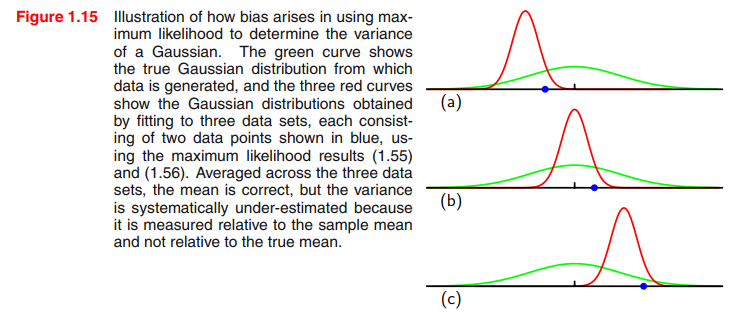
\includegraphics[width=0.8\linewidth]{fig/biased_ML_Gaussian.png}
\end{figure}

而\textbf{样本协方差矩阵}的无差估计如下
\[C=\frac{1}{n-1}\sum_{k=1}^n(\vx_k-\hat{\vmu})(\vx_k-\hat{\vmu})^\T\]

\subsection{贝叶斯参数估计}
在最大似然估计方法中,将需要估计的参数向量$\vtheta$看作一个确定而未知的参数,而在贝叶斯方法中,我们将参数向量$\vtheta$\textbf{本身看作一个随机变量},已有的训练样本可以使我们把对于$\vtheta$的初始密度估计(先验)转为后验概率密度。

\begin{figure}[H]
\centering
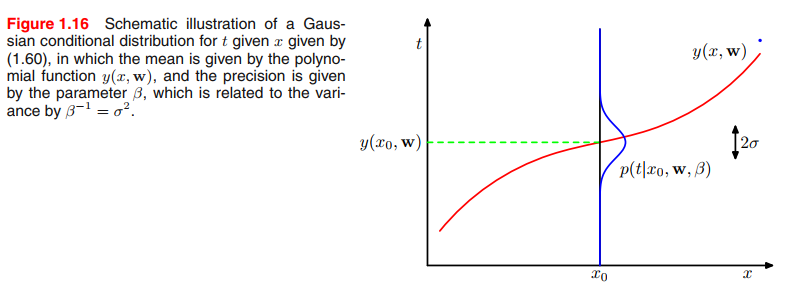
\includegraphics[width=0.8\linewidth]{fig/bayesian_est.png}
\end{figure}
% 将训练样本依据类别归到$c$个次样本集$\mD_1,\ldots,\mD_c$中,结合先验,贝叶斯公式可表成
% \[P(\omega_i\mid\vx)=\frac{p(\vx\mid\omega_i,\mD_i)P(\omega_i)}{\sum_{j=1}^cp(\vx\mid\omega_j,\mD_j)P(\omega_j)}\]

已知训练样本$\mD$,这些样本都从固定但未知的概率密度函数$p(\vx)$中独立抽取,要求根据这些样本估计$p(\vx\mid\mD)$,即贝叶斯学习的核心问题。

得到贝叶斯估计的核心公式(Gibbon)
\[\begin{aligned}
p(\vx\mid\mD)&=\int p(\vx,\vtheta\mid\mD)\diff\vtheta
=\int p(\vx\mid\vtheta,\mD)p(\vtheta\mid\mD)\diff\vtheta\\
&=\int p(\vx\mid\vtheta)p(\vtheta\mid\mD)\diff\vtheta
\end{aligned}\]
后一式成立的原因是测试样本$\vx$和训练样本集$\mD$的选取是独立进行的。
根据贝叶斯公式
\[p(\vtheta\mid\mD)=\frac{p(\mD\mid\vtheta)p(\vtheta)}{\int p(\mD\mid\vtheta)p(\vtheta)\diff\vtheta}=\alpha\prod_{k=1}^np(\vx_k\mid\vtheta)p(\vtheta)\]
其中$\alpha$是一个依赖于样本集$\mD$的归一化系数,不依赖于$\vtheta$。

当先验$p(\vtheta)$为高斯密度时,$p(\vtheta\mid\mD)$依然为正态分布,称为再生(reproducing)函数,将$p(\vtheta)$称为共轭(conjugate)先验。

考虑样本数不断增加的过程
\[p(\vtheta\mid\mD^n)=\frac{p(\vx_n\mid\vtheta)p(\vtheta\mid\mD^{n-1})}{\int p(\vx_n\mid\vtheta)p(\vtheta\mid\mD^{n-1})\diff\vtheta}\]
当没有观测样本时,$p(\vtheta\mid\mD^0)=p(\vtheta)$,反复应用上述公式有概率密度函数$p(\vtheta),p(\vtheta\mid\vx_1),p(\vtheta\mid\vx_1,\vx_2)$等,实际上即增量学习(incremental learning)。

而最大后验(maximum a posteriori, MAP)则是使$p(\mD\mid\vtheta)p(\vtheta)$取最大值的参数向量$\vtheta$,这里通常先乘起来再取对数
\[\argmax_{\vtheta} \lrp{\ln p(\mD\mid\vtheta) + \ln p(\vtheta)}
=\lrp{\sum_{k=1}^n\ln p(\vx_k\mid\vtheta)+\ln p(\vtheta)}\]

可以比较最大似然与贝叶斯之间的差异。
\begin{center}
\begin{tabular}{|c|c|c|}\hline
 & 最大似然 & 贝叶斯\\\hline
估计对象 & 单一参数 & 完整分布\\\hline
计算复杂度 & 微分 & 多重积分\\\hline
可理解性 & 确定易理解 & 不确定不易理解\\\hline
先验的准确程度 & 不准确 & 准确\\\hline
\end{tabular}
\end{center}

% \subsection{维数问题}
% 引入新的特征
% 计算复杂度
% 过拟合
% PCA

\subsection{Fisher线性判别}
PCA方法寻找的是用来有效表示的主轴方向,而判别分析方法(discriminant analysis)寻找的是用来有效\textbf{分类}的方向。

考虑将$d$维空间中的数据点投影到一条直线上,以最大限度区分各类数据点的投影方向。
假设有一组$n$个$d$维的样本$\vx_1,\ldots,\vx_n$分属两个不同类别,其中$n_1$个样本的子集$\mD_1$属于$\omega_1$,$n_2$个样本的子集$\mD_2$属于$\omega_2$。
对$\vx$中各个成分做线性组合,得到点积\footnote{回忆高中知识,点积相当于做投影,将$\vx$往直线$\vw$上投影}$y=\vw^\T\vx$,进而全部$n$个样本产生$n$个结果$y_1,\ldots,y_n$相应属于$\mY_1$和$\mY_2$。
\begin{figure}[H]
\centering
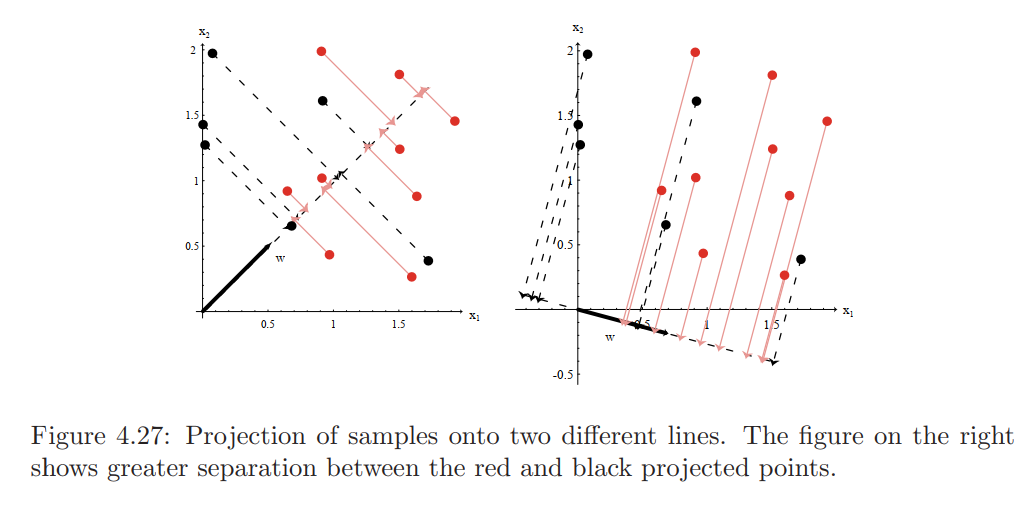
\includegraphics[width=0.8\linewidth]{fig/Fisher.png}
\end{figure}

如何确定最佳的直线方向$\vw$得到最佳的分类效果,一个衡量标准即样本均值的差。
设原样本第$i$个类别的均值为$\vm_i$,则投影后的样本均值为$\tilde{\vm}_i=\vw^\T\vm_i$。
样本均值之差为
\[|\tilde{\vm}_1-\tilde{\vm}_2|=|\vw^\T(\vm_1-\vm_2)|\]
可以通过$\vw$幅值方法来得到任意大小的均值之差,但这样子没有意义。
因此定义类别$\omega_i$的类内散布(scatter)/方差如下
\[\tilde{s}_i^2=\sum_{y\in\mY_i}(y-\tilde{m})^2\]
这样$1/n(\tilde{s}_1^2+\tilde{s}_2^2)$即为全部数据总体方差的估计,$\tilde{s}_1^2+\tilde{s}_2^2$称为投影样本的总类内散布。

故Fisher线性可分性准则要求在投影$y=\vw^\T\vx$下
\[\max_{\vw} J(\vw):=\frac{|\tilde{m}_1-\tilde{m}_2|^2}{\tilde{s}_1^2+\tilde{s}_2^2}\]
即均值差尽可能大,同时类内方差尽可能小。

定义类内散布矩阵$S_i$和总类内散布矩阵$S_W$如下
\[\begin{aligned}
S_i &= \sum_{\vx\in\mD_i}(\vx-\vm_i)(\vx-\vm_i)^\T\\
S_W &= S_1+S_2
\end{aligned}\]
可求得
\[\begin{aligned}
\tilde{s}_i^2 &= \vw^\T S_i\vw\\
\tilde{s}_1^2+\tilde{s}_2^2 &= \vw^\T S_W\vw\\
\end{aligned}\]
而投影样本均值之差
\[\begin{aligned}
S_B &= (\vm_1-\vm_2)(\vm_1-\vm_2)^\T\\
(\tilde{\vm}_1-\tilde{\vm}_2)^2 &= \vw^\T S_B\vw
\end{aligned}\]
其中$S_B$称为总类间散布矩阵。
$S_W$和$S_B$都是对称且半正定的。

进而原来的准则函数可写成
\[J(\vw)=\frac{\vw^\T S_B\vw}{\vw^\T S_W\vw}\]
称为广义瑞利商,可证令其最大化
\[S_B\vw=\lambda S_W\vw\]
一般情况下
\[\argmax_{\vw}J(\vw)=S_W^{-1}(\vm_1-\vm_2)\]
% !TEX root = main.tex

\section{非参数技术} % 4.1-4.6
% Parzen窗 p_n(x)=(k_n/n)/V_n=...

\subsection{概率密度的估计}
向量$\vx$落在区域$\mR$的概率为
\[P=\int_{\mR}p(\vx')\diff\vx'\]
即$P$是概率密度函数$p(\vx)$平滑后的版本。
若假设$p(\vx)$是连续的,且区域$\mR$足够小,以致于在这个区间中$p$几乎没有变化,则
\[\int_{\mR}p(\vx')\diff\vx'\approx p(\vx) V\]
其中$\vx$为一个点,而$V$为区域$\mR$所包含的体积。
可以用下述公式作为一个估计
\[p(\vx)\approx\frac{k/n}{V}\]
即从$n$个服从$p(\vx)$的独立同分布样本落在$\mR$中的有$k$个。

为了估计$\vx$的概率密度函数,构造一系列包含$\vx$的区域$\mR_1,\mR_2,\ldots$,第一个区域用$1$个样本,第二个区域用$2$个,以此类推。
$V_n$为区域$\mR_n$的体积,$k_n$为落在区间$\mR_n$中的样本个数,而$p_n(\vx)$表示对$p(\vx)$的第$n$次估计:
\[p_n(\vx)=\frac{k_n/n}{V_n}\]
若要求$p_n(\vx)$能够收敛到$p(\vx)$,则下面3个条件必须满足:
\begin{itemize}
	\item $\lim_{n\to\infty}V_n=0$
	\item $\lim_{n\to\infty}k_n=\infty$
	\item $\lim_{n\to\infty}k_n/n=0$
\end{itemize}
第一个条件保证区域均匀收缩和$p(\cdot)$在点$\vx$处连续的情况下,区间平滑了的$P/V$能够收敛到$p(\vx)$。
第二个条件只有在$p(\vx)\ne 0$才有意义,保证频率之比能够收敛到概率$P$。
最后一个条件说明虽然最后落在小区域$\mR_n$中的样本数目非常大,但是这么多样本在全体样本中所占的比例非常小。
这里通常考虑均方意义下的收敛\footnote{\url{https://en.wikipedia.org/wiki/Convergence_of_random_variables}}。

\subsection{Parzen窗方法}
假设区间$\mR_n$是$d$维超立方体,$h_n$为一条边长度,体积为
\[V_n=h_n^d\]
定义窗函数
\[\varphi(\vu)=\begin{cases}
1 & |\vu_j|\leq 1/2,\;j=1,\ldots,d\\
0 & \text{其他}
\end{cases}\]
这样$\varphi(\vu)$就表示一个中心在原点的单位超立方体。
若$\vx_i$落在中心点为$\vx$的立方体$V_n$中,那么
\[\varphi\lrp{\frac{\vx-\vx_i}{h_n}}=1\]
否则为$0$,进而可解析表达超立方体样本个数
\[k_n=\sum_{i=1}^n\varphi\lrp{\frac{\vx-\vx_i}{h_n}}\]
代入估计式有
\[p_n(\vx)=\frac{1}{n}\sum_{i=1}^n\frac{1}{V_n}\varphi\lrp{\frac{\vx-\vx_i}{h_n}}\]

均值的收敛性
\[\begin{aligned}
\bar{p}_n(\vx)&=\E{p_n(\vx)}\\
&=\frac{1}{n}\sum_{i=1}^n\E{\frac{1}{V_n}\varphi\lrp{\frac{\vx-\vx_i}{h_n}}}\\
&=\int\frac{1}{V_n}\varphi\lrp{\frac{\vx-\vx_i}{h_n}}p(\vv)\diff\vv\\
&=\int\delta_n(\vx-\vv)p(\vv)\diff\vv
\end{aligned}\]

\subsection{$k_n$近邻估计}
最佳的窗函数的选择是个问题,因此一种可行的方案是让体积成为训练样本的函数,而不是硬性规定窗函数为样本个数的某个函数。

比如说可以取$k_n=\sqrt{n}$,有下列迭代过程。
\begin{figure}[H]
\centering
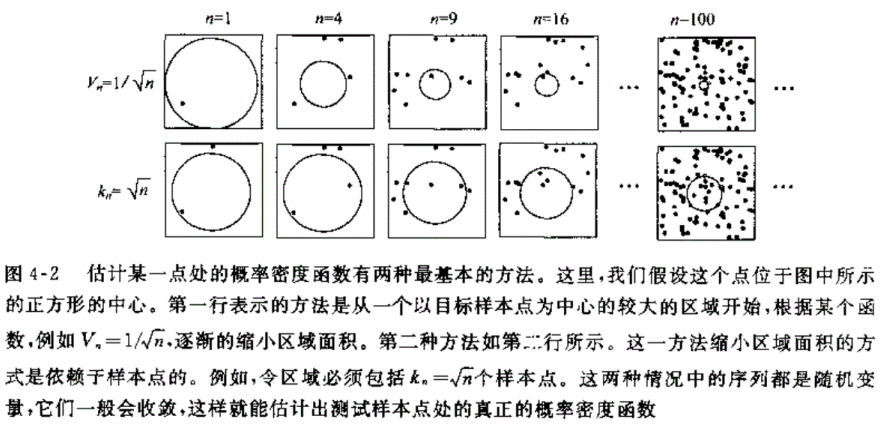
\includegraphics[width=0.8\linewidth]{fig/kn-neighbor.png}
\end{figure}

\subsection{最近邻规则}
\begin{figure}[H]
\centering
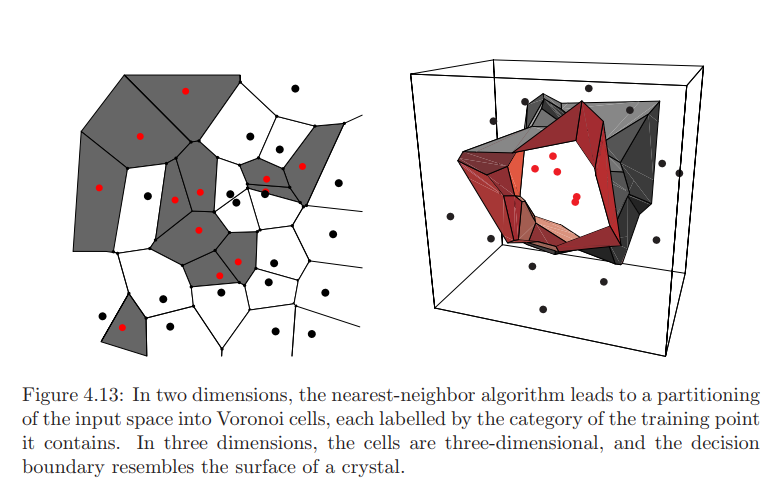
\includegraphics[width=0.8\linewidth]{fig/nearest_neighbors.png}
\end{figure}

定义$\omega_m(\vx)$为
\[P(\omega_m\mid\vx)=\max_i P(\omega_i\mid\vx)\]
令$P^*(e\mid\vx)$表示$P(e\mid\vx)$的最小可能值,$P^*$为$P(e)$的最小可能值,则根据贝叶斯风险
\[P^*(e\mid\vx)=1-P(\omega_m\mid\vx)\]
有总的误差率
\[P^*=\int P^*(e\mid\vx)p(\vx)\diff\vx\]
记$n$个样本的平均误差率为$P_n(e)$,且
\[\begin{aligned}
P&=\lim_{n\to\infty}P_n(e)\\
&=\lim_{n\to\infty}\int P_n(e\mid\vx)p(\vx)\diff\vx\\
&=\int\lrs{1-\sum_{i=1}^cP^2(\omega_i\mid\vx)}p(\vx)\diff\vx
\end{aligned}\]
可以证明
\[P^*\leq P\leq P^*\lrp{2-\frac{c}{c-1}P^*}\]
\begin{figure}[H]
\centering
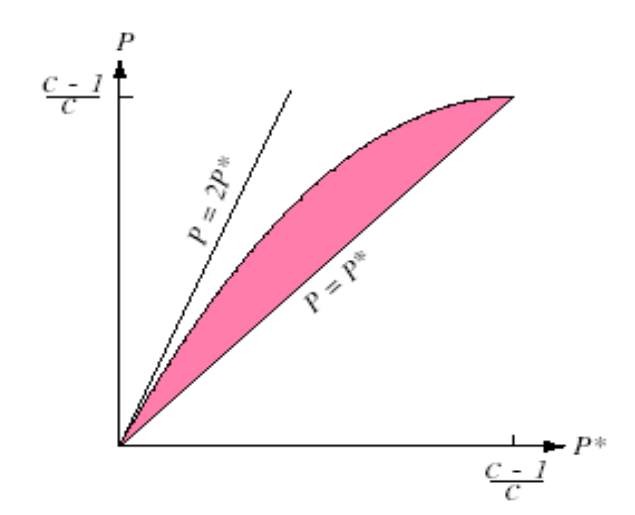
\includegraphics[width=0.4\linewidth]{fig/kNN_error_bound.png}
\end{figure}

进而推广有$k$近邻规则(KNN)。
% !TEX root = main.tex

\section{线性判别函数} % 5.1-5.8 (5.10-5.12)
% 5.2 线性判别函数和判定面(单类、多类)
% 广义线性判别函数 5.3
% 5.4 两类线性可分情况
%  梯度下降法、牛顿法、Hessian矩阵
% 感知器算法 5.5
% 5.6 松弛算法
% 5.7 不可分情况
% MSE 5.8
%  MSE与Fisher线性判别
% 5.10 线性规划
% SVM 5.11
%  VC Dimension
%  Kernel Trick
%  Soft Margin
% 5.12 拓展到多类
% Model Selection
%  Cross Validation (k-fold)

\subsection{线性判别函数和判定面}
判别(discriminant)函数是指由$\vx$的各个分量线性组合而成的函数
\[g(\vx)=\vw^\T\vx+w_0\]
这里$\vw$是权向量,$w_0$称为阈权值(threshold)或偏置。

对于二类线性分类器来说,$g(\vx)>0$则判为$\omega_1$,否则判为$\omega_2$。
方程$g(\vx)=0$定义了一个判定面,将归类于$\omega_1$和$\omega_2$的点分开来。
当$g(\vx)$是线性的,这个平面称为超平面。

判别函数是特征空间某点$\vx$到超平面距离的代数度量(注意到垂直平行特性)
\[\vx=\vx_p+r\frac{\vw}{\norm{\vw}}\]
其中$\vx_p$是$\vx$在超平面$H$上的投影向量,$r$是相应的算术距离,为正则$\vx$在$H$正侧,否则在$H$负侧。
由于$g(\vx_p)=0$,有
\[g(\vx)=\vw^\T\vx+w_0=r\norm{\vw}\]
或
\[r=\frac{g(\vx)}{\norm{\vw}}\]
\begin{figure}[H]
\centering
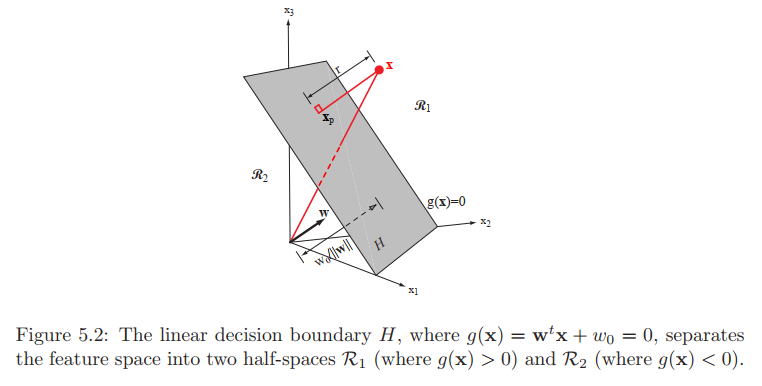
\includegraphics[width=0.9\linewidth]{fig/linear_decision_boundary.png}
\end{figure}

对于多类样本来说,则将$c$类问题转化为$c$个二类问题;或者用$c(c-1)/2$个线性判别函数,将样本分为$c$个类别,每个线性判别函数只对其中两个类别分类。

\subsection{广义线性判别函数}
线性判别函数可写成
\[g(\vx)=w_0+\sum_{i=1}^d w_i x_i\]
系数$w_i$是权向量$\vw$的分量,通过加入另外的项($\vw$的各对分量之间的乘积),得到二次判别函数
\[g(\vx)=w_0+\sum_{i=1}^d w_ix_i+\sum_{i=1}^d\sum_{j=1}^d w_{ij}x_ix_j\]
因$x_ix_j=x_jx_i$,不失一般性假设$w_{ij}=w_{ji}$。

继续加入更高次项(如$w_{ijk}x_ix_jx_k$)可得到多项式判别函数,可看作对某一判别函数$g(x)$做级数展开,然后取截尾逼近,意味着某一广义线性判别函数
\[g(\vx)=\sum_{i=1}^d a_iy_i(\vx)\]
或
\[g(\vx)=\va^\T\vy\]

特别地,线性判别函数可写成
\[g(\vx)=w_0+\sum_{i=1}^d w_i x_i=\sum_{i=0}^dw_ix_i\]
令$\vy=\bmat{1 & \vx}^\T$为\textbf{增广特征向量},$\va=\bmat{w_0 & \vw}$为增广权向量,注意这里是将偏置放在了第$0$位。

对于一个样本$\vy_i$,若$\va^\T\vy_i>0$就标记为$\omega_1$,若$\va^\T\vy_i<0$就标记为$\omega_2$。
这样可以通过一种规范化(normalization)方法来简化两类样本训练过程,即对于属于$\omega_2$的样本,用负号表示而不是标记$\omega_2$(将属于$\omega_2$的样本用$\bmat{-1 & -y_i}^\T$表示)。
这样就可以直接寻找一个对所有样本都有$\va^\T\vy_i>0$的权向量$\va$,这样的向量称为分离(separating)向量或解向量。

求解权向量的过程相当于确定权空间中一点,每个样本都对应解向量的可能位置给出限制。
$\va\vy_i^\T$确定了一个穿过权空间原点的超平面,$\vy_i$为其法向。
解向量若存在,则一定在每个超平面的正侧。
由于是不等式约束,故解不唯一,要加入其他约束条件。
一种方法是找到一个单位长度的权向量,使得从样本到分类平面最小距离达到最大;另一种方法则在所有$i$中寻找满足$\va^\T\vy_i\geq b$的具有最小长度的权向量,这里的$b$是被称为边沿裕量(margin)/间隔的正常数。

求解$\va^\T\vy_i>0$的解所采用的方法是:定义一个准则函数$J(\va)$,当$\va$是解向量时,$J(\va)$最小,因此可将其简化为一个标量函数极小化问题,通常用梯度下降法解决。
\[\va(k+1)=\va(k)-\eta(k)\nabla J(\va(k))\]
其中$\eta$为正的比例因子,即学习率。

假设准则函数可以通过二阶展开近似
\[J(\va)\approx J(\va(k))+\nabla J^\T(\va-\va(k))+\frac{1}{2}(\va-\va(k))^\T H(\va-\va(k))\]
即当选择
\[\eta(k)=\frac{\norm{\nabla J}^2}{\nabla J^T H\nabla J}\]
时,可使$J(\va(k+1))$最小化。

牛顿法
\[\va(k+1)=\va(k)-H^{-1}\nabla J\]

\subsection{感知器}
考虑构造线性不等式$\va^\T\vy_i>0$的准则函数,用错分的样本作为准则函数不好因为分段常数不利于梯度搜索。
更好的选择是感知器(perceptron)准则函数
\[J_p(\va)=\sum_{\vy\in\mY}(-\va^\T\vy)\]
这里$\mY(\va)$是被$\va$错分的样本集。
由几何上知,$J_p(\va)$是与错分样本到判决边界距离之和成正比的。
对上式求导有
\[\nabla J_p=\sum_{\vy\in\mY}(-\vy)\]
得到梯度下降迭代公式
\[\va(k+1)=\va(k)+\eta(k)\sum_{\vy\in\mY_k}\vy\]

\subsection{最小平方误差}
设$Y$为$n\times\hat{d}$的矩阵,$n$为样本数,$\hat{d}=d+1$为维度,第$i$行是向量$\vy_i^\T$,令$\vb=\bmat{b_1 &\cdots & b_n}^\T$,目标是找到权重$\va$满足
\[Y\va=\vb\]
定义误差向量
\[\ve=Y\va-\vb\]
使误差向量长度平方最小化,即最小化平方误差和(MSE)准则函数
\[J_s(\va)=\norm{Y\va-\vb}^2=\sum_{i=1}^n(\va^\T\vy_i-b_i)^2\]
计算梯度有
\[\nabla J_s=2Y^\T(Y\va-\vb)\]
令其为$0$有
\[Y^\T Y\va=Y^\T\vb\]
当方阵$Y^\T Y$非奇异时,有唯一解
\[\va=(Y^\T Y)^{-1} Y^\T\vb=Y^\dag\vb\]
这里的$\hat{d}\times n$矩阵
\[Y^\dag=(Y^\T Y)^{-1} Y^\T\]
称为$Y$的伪逆矩阵。
注意到若$Y$为方阵且非奇异,则这个伪逆矩阵即为$Y$的逆矩阵。
还应注意到$Y^\dag Y=I$,但通常$YY^\dag\ne I$。

MSE与Fisher线性判别函数的解是一样的。

\subsection{支持向量机}
支持向量机(support vector machine, SVM)通过一个足够高维的非线性映射$\varphi(\cdot)$,将两类数据用超平面进行分割。
假设每个模式$\vx_k$变换到$\vy_k=\varphi(\vx_k)$,则问题在于选择$\varphi(\cdot)$。
对$n$个模式中的每一个$k=1,\ldots,n$,根据模式属于$\omega_1$或$\omega_2$,分别令$z_k=\pm 1$,增广空间$\vy$上的判别函数是
\[g(\vy)=\va^\T\vy\]
这里权向量和变换后的模式向量都是增广的(取$a_0=w_0,y_0=1$),则这样的分割超平面保证
\[z_kg(\vy_k)\geq 1,\;k=1,\ldots,n\]
\begin{figure}[H]
\centering
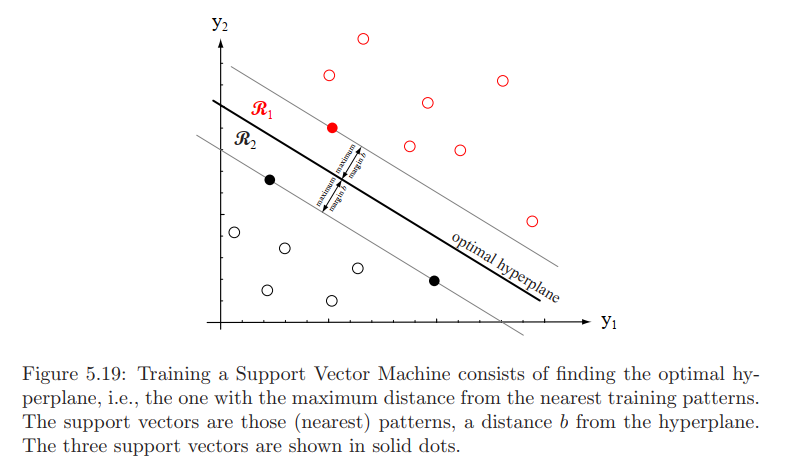
\includegraphics[width=0.9\linewidth]{fig/SVM.png}
\end{figure}

训练一个支持向量机的目标是找到一个具有\textbf{最大间隔}(largest margin)的分割平面,若间隔越大则得到的分类器也越好。
从超平面到变换后的模式$\vy$的距离是$|g(\vy)|/\norm{\va}$(即做投影),若正的间隔$b$存在,则推出
\[\frac{z_kg(\vy_k)}{\norm{\va}}\geq b,\;k=1,\ldots,n\]
目标即找一个使得$b$最大化的权向量$\va$。
由于解向量可以任意伸缩且保持超平面不变,故有限制条件$b\norm{a}=1$,即其确定的是$\norm{\va}$的极小值。

支持向量是使上式等号成立的模式向量,即支持向量是最靠近超平面的,也是最难分类的样本/对求解分类任务最富有信息的模式。

目标为极小化$\norm{\va}$,构造拉格朗日函数
\[L(\va,\valpha)=\frac{1}{2}\norm{\va}^2-\sum_{k=1}^n\alpha_k[z_k\va^\T\vy_k-1]\]
可用KKT条件改写为
\[\begin{aligned}
&L(\valpha)=\sum_{i=1}^n\alpha_i-\frac{1}{2}\sum_{k,j}^n\alpha_k\alpha_jz_kz_j\vy_j^\T\vy_k\\
&s.t.\sum_{k=1}^nz_k\alpha_k=0,\;\alpha_k\geq 0,\;k=1,\ldots,n
\end{aligned}\]
进行求解(先用约束消元,逐一令偏导为$0$求解)。

\subsection{软间隔与正则化}
前面都假定训练样本在样本空间或特征空间中线性可分,然而现实中却很难找到这些线性可分的任务,也很难判定不是由于过拟合造成。
缓解该问题一个方法是允许支持向量机在一些样本上出错,为此引入软间隔(soft margin)概念。
\begin{figure}[H]
\centering
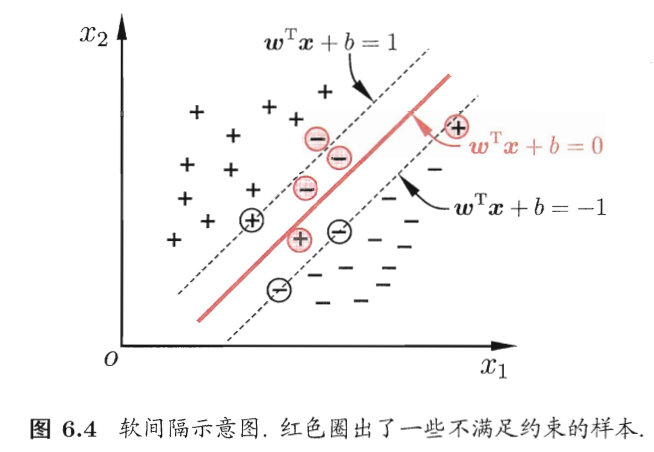
\includegraphics[width=0.6\linewidth]{fig/soft_margin.png}
\end{figure}

允许某些样本不满足不等式约束
\[y_i(\vw^\T\vx_i+b)\geq 1\]
于是在最大化间隔的同时,不满足约束的样本应尽可能少,得到优化目标
\[\min_{\vw,b}\frac{1}{2}\norm{\vw}^2+C\sum_{i=1}^ml_{0/1}(y_i(\vw^\T\vx+b)-1),\,C>0\]
其中$l_{0/1}$为0/1损失函数。

也有其他损失函数
\begin{itemize}
	\item Hinge损失:$l_{hinge}(z)=\max(0,1-z)$
	\item 指数损失:$l_{exp}(z)=\exp(z)$
	\item 对率损失:$l_{log}(z)=\log(1+\exp(-z))$
\end{itemize}

\subsection{核方法}
对变量升维,以便线性划分
\[\kappa(\vx,\vx_i)=\phi(\vx_i)^\T\phi(\vx)\]

\subsection{VC维}
衡量函数复杂性,通过评估函数类中函数的弯曲程度实现。
VC维越大,曲线越弯曲。
\begin{figure}[H]
\centering
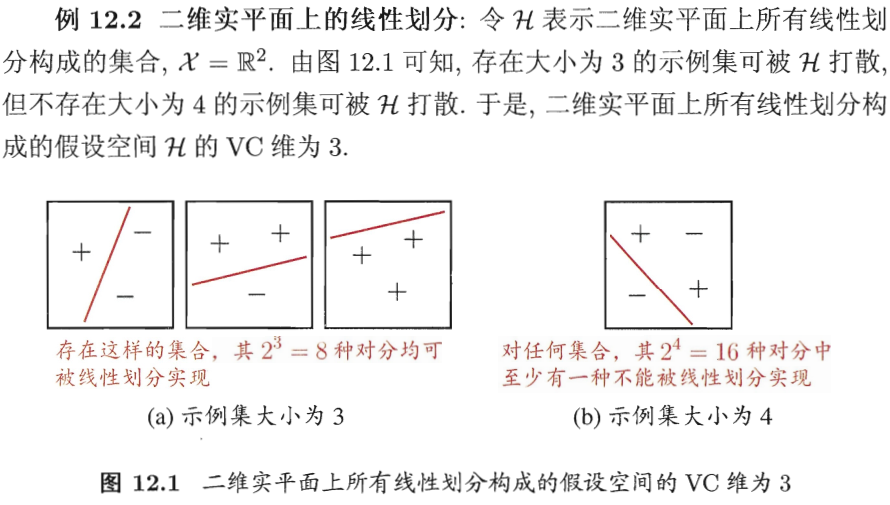
\includegraphics[width=0.6\linewidth]{fig/vc_dimension.png}
\end{figure}
% !TEX root = main.tex

\section{多层神经网络}
三层神经网络:输入层、隐含层、输出层,也称多层感知器(multilayer perceptron, MLP)
\begin{figure}[H]
\centering
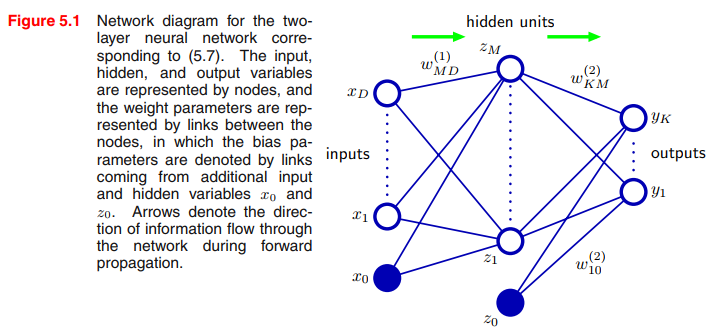
\includegraphics[width=0.8\linewidth]{fig/forward_propagation.png}
\end{figure}

前馈运算如下,判别函数$y_k(\vx,\vw)$为每个输出单元产生的信号
\[y_{k}(\mathbf{x}, \mathbf{w})=\sigma\left(\sum_{j=1}^{M} w_{k j}^{(2)} h\left(\sum_{i=1}^{D} w_{j i}^{(1)} x_{i}+w_{j 0}^{(1)}\right)+w_{k 0}^{(2)}\right)\]

任何从输入到输出的连续映射函数都可以用一个三层非线性网络实现,只要有足够的隐单元$M$、适当的非线性函数和权值。

最小化误差函数
\[E(\mathbf{w})=\frac{1}{2} \sum_{n=1}^{N}\left\|\mathbf{y}\left(\mathbf{x}_{n}, \mathbf{w}\right)-\mathbf{t}_{n}\right\|^{2}\]


% !TEX root = main.tex

\section{随机方法} % 7.1-7.3 (7.4-7.5)
假设给定多个变量$s_i$,其中每个变量数值都取两个离散值之一,记为$\pm 1$。
优化问题为确定$N$个$s_i$的合适取值,使下述代价函数或能量函数最小
\[E=-\frac{1}{2}\sum_{i,j=1}^N w_{ij}s_is_j\]
其中$w_{ij}$是对称的,取值可正可负。
\begin{figure}[H]
\centering
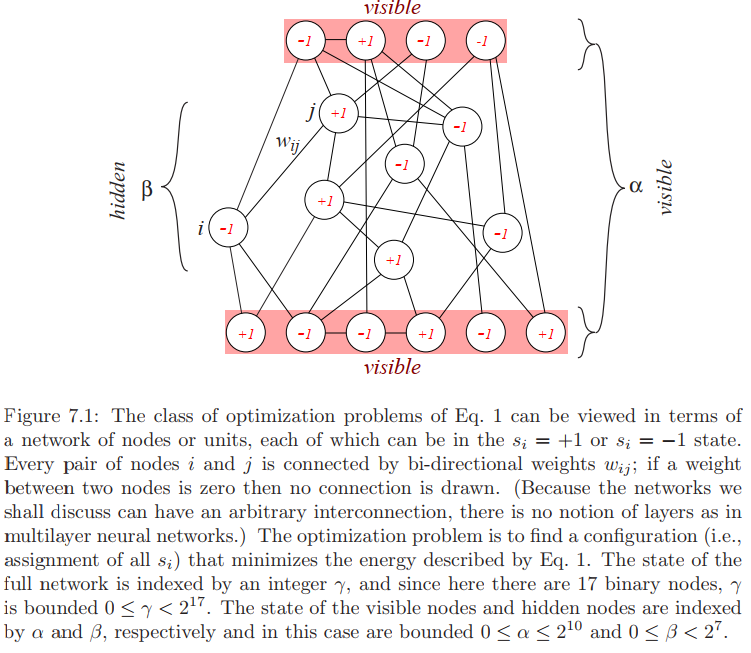
\includegraphics[width=0.9\linewidth]{fig/stochastic_opt_problem.png}
\end{figure}

\subsection{模拟退火}
一个系统具有能量$E_\gamma$通过下式给出
\[P(\gamma)=\frac{\ee^{-E_\gamma/T}}{Z(T)}\]
其中分子为Boltzmann因子,而$Z$是一个归一化常量/分配(partition)函数
\[Z(T)=\sum_{\gamma'}\ee^{-E_{\gamma'}/T}\]
为Boltzmann因子对所有构型的求和。

\begin{algorithm}[H]
\caption{模拟退火(Simulated Annealing)}
\begin{algorithmic}[2]
\State 将网络随机初始化,并设一个高的初始温度$T(1)$
\State 随机选择节点$i$,设其状态为$s_i=+1$,计算该构型下系统总能量$E_a$
\State 改变其道候选状态不$s_i=-1$,系统总能量为$E_b$
\If{$E_b<E_a$}
\State 接受此次状态改变
\Else
\State 以$\ee^{-\Delta E_{ab}/T}$概率接受改变,其中$\Delta E_{ab}=E_b-E_a$
\EndIf
\end{algorithmic}
\end{algorithm}
\begin{figure}[H]
\centering
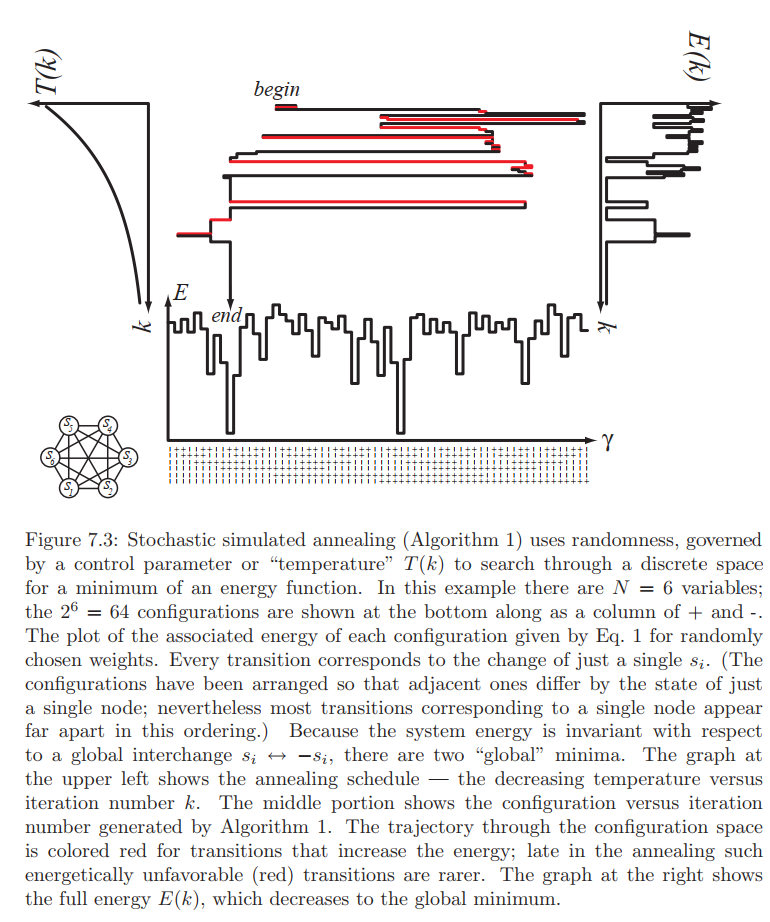
\includegraphics[width=0.8\linewidth]{fig/simulated_annealing.png}
\end{figure}

\subsection{Boltzmann学习}
\begin{figure}[H]
\centering
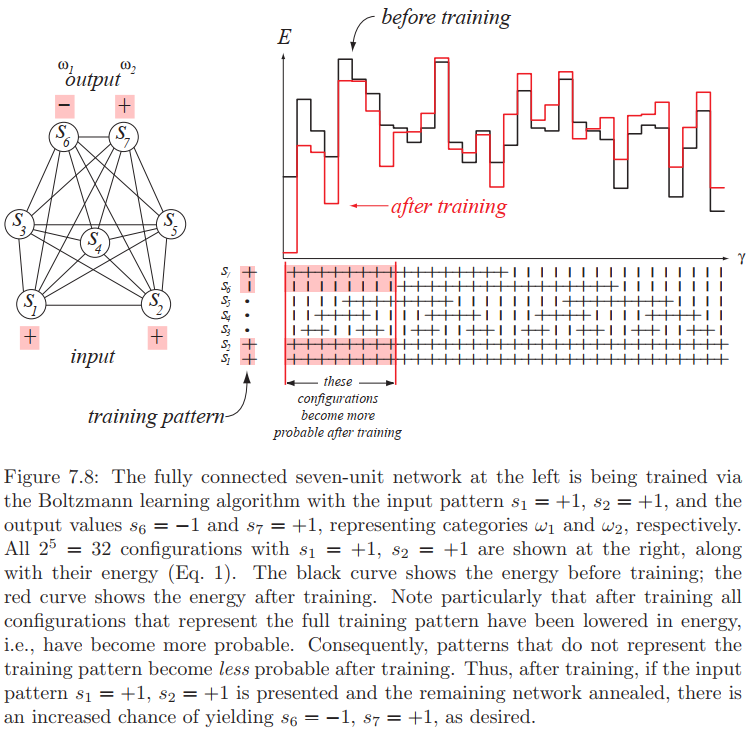
\includegraphics[width=0.8\linewidth]{fig/boltzmann_learning.png}
\end{figure}

\end{document}

% ftp://222.200.180.156/
% student
% 2019s

% 1.1-1.6
% 2.1-2.9 (2.10-2.11)
% 3.1-3.5 3.7-3.8 (3.9)
% 4.1-4.6
% 5.1-5.8 (5.10-5.12)
% 6.1-6.6 6.8 (6.9)
% 7.1-7.3 (7.4-7.5)
% (10.1-10.9)